\documentclass[a4paper, 12pt]{extarticle}
\usepackage[top=1in, bottom=1in, left=1in, right=1in]{geometry}
\usepackage{amsmath}
\usepackage{amssymb}
\usepackage{graphicx}
\usepackage{fontspec}
\usepackage{tikz}
\usepackage{amsmath}
\usepackage{amssymb}
\usepackage{enumitem}
\usepackage{booktabs}
\usepackage{tcolorbox}
\usepackage{fontspec}
\usepackage{hyperref}
\usepackage{tikz}
\usepackage{fontspec}
%\usetikzlibrary{decorations.pathmorphing}
\usetikzlibrary{calc,decorations,patterns,arrows,decorations.pathmorphing,positioning}
\definecolor{pltblue}{HTML}{1F77B4}
\tikzset{every picture/.style={/utils/exec={\fontspec{Pretty Neat}}}}
\setmainfont{Pretty Neat}


\makeatletter
\pgfset{
  /pgf/decoration/randomness/.initial=2,
  /pgf/decoration/wavelength/.initial=100
}
\pgfdeclaredecoration{sketch}{init}{
  \state{init}[width=0pt,next state=draw,persistent precomputation={
    \pgfmathsetmacro\pgf@lib@dec@sketch@t0
  }]{}
  \state{draw}[width=\pgfdecorationsegmentlength,
  auto corner on length=\pgfdecorationsegmentlength,
  persistent precomputation={
    \pgfmathsetmacro\pgf@lib@dec@sketch@t{mod(\pgf@lib@dec@sketch@t+pow(\pgfkeysvalueof{/pgf/decoration/randomness},rand),\pgfkeysvalueof{/pgf/decoration/wavelength})}
  }]{
    \pgfmathparse{sin(2*\pgf@lib@dec@sketch@t*pi/\pgfkeysvalueof{/pgf/decoration/wavelength} r)}
    \pgfpathlineto{\pgfqpoint{\pgfdecorationsegmentlength}{\pgfmathresult\pgfdecorationsegmentamplitude}}
  }
  \state{final}{}
}
\tikzset{xkcd/.style={decorate,decoration={sketch,segment length=0.5pt,amplitude=0.5pt}}}
\makeatother

\usepackage{etoolbox}
\AtBeginEnvironment{tabular}{\fontspec{Pretty Neat}}

\setlength{\parindent}{0pt}
\setlength{\parskip}{0.5em}
\usepackage{fancyhdr}
\usepackage{geometry}
\usepackage{adjustbox}
\usepackage{titling}
\usepackage{multicol}
\usepackage{amsmath}
\usepackage{amssymb}
\usepackage{graphicx}
\usepackage{hyperref}
\usepackage{tikz}
\usepackage{fontspec}
\usetikzlibrary{calc,decorations,patterns,arrows,decorations.pathmorphing}
\definecolor{pltblue}{HTML}{1F77B4}

\usepackage{amsmath}
\usepackage{tikz}
\usepackage{enumitem}

\title{Random Walk Characteristics Worksheet}
\author{Network Science Course}
\date{}

\begin{document}

\section{Image Processing and Convolution}

\subsection{Preparation: Understanding Convolution}
Think of convolution as a way to find patterns in an image by looking through a small window (kernel). As we slide this window across the image, we:
\begin{enumerate}
    \item Look at a small neighborhood of pixels
    \item Multiply each pixel by the corresponding value in our pattern-matching window (kernel)
    \item Sum up these products to get a single number
    \item Move the window and repeat
\end{enumerate}

For example, if we want to detect vertical edges, we might use this kernel:
\[
K = \begin{bmatrix}
-1 & 1 & 0 \\
-1 & 1 & 0 \\
-1 & 1 & 0
\end{bmatrix}
\]

Let's see how it works on a small image region (3x3 pixels):

\[
\begin{bmatrix}
10 & 80 & 10 \\
10 & 80 & 10 \\
10 & 80 & 10
\end{bmatrix}
\]

We multiply each pixel by the corresponding kernel value and sum: $(10 \times -1 + 80 \times 1 + 10 \times 0) \times 3 = 210$. The high positive value (210) indicates a strong vertical edge was detected.
Here are some common kernel patterns:

\textbf{Vertical edge detection:}
\[
\begin{bmatrix}
-1 & 1 & 0 \\
-1 & 1 & 0 \\
-1 & 1 & 0
\end{bmatrix}
\quad
\text{Looks for } \xrightarrow{\text{dark to bright}}
\]

\textbf{Horizontal edge detection:}
\[
\begin{bmatrix}
-1 & -1 & -1 \\
1 & 1 & 1 \\
0 & 0 & 0
\end{bmatrix}
\quad
\text{Looks for } \downarrow \text{ dark to bright}
\]

\textbf{Blur/Smoothing:}
\[
\frac{1}{9}\begin{bmatrix}
1 & 1 & 1 \\
1 & 1 & 1 \\
1 & 1 & 1
\end{bmatrix}
\quad
\text{Averages all neighboring pixels}
\]

\clearpage

\subsection{Image Processing and Convolution}

Consider a 6x6 grayscale image showing a diagonal line pattern:

\begin{center}
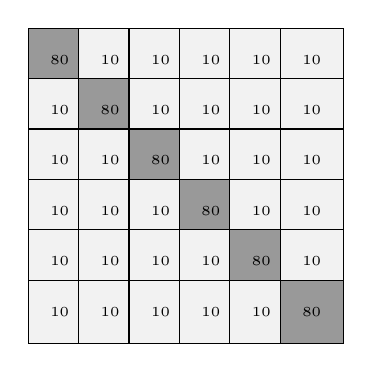
\begin{tikzpicture}[scale=0.8]
    % Create 6x6 grid
    \foreach \i in {0,...,5} {
        \foreach \j in {0,...,5} {
            \pgfmathsetmacro{\value}{ifthenelse(\i==\j, 80, 10)}
            \node[rectangle, draw, minimum size=0.8cm, fill=gray!\value] at (\i*0.8, -\j*0.8) {\tiny \value};
        }
    }
\end{tikzpicture}
\end{center}

\begin{enumerate}
\item If we want to detect diagonal edges, which kernel of size 3x3 would be most appropriate? The kernel should have the values between -1 and 1.
\begin{center}
    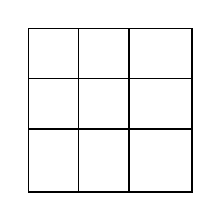
\begin{tikzpicture}[scale=0.8]
        % Create 6x6 grid
        \foreach \i in {0,...,2} {
            \foreach \j in {0,...,2} {
                \pgfmathsetmacro{\value}{ifthenelse(\i==\j, 10, 10)}
                \node[rectangle, draw, minimum size=0.8cm, fill=white] at (\i*0.8, -\j*0.8) {};
            }
        }
    \end{tikzpicture}
\end{center}

\item Apply your kernel to compute the convoluted image. No need to calculate the value of each pixel exactly but show your estimate by shading the pixels. For the boundary pixels, leave them blank since the kernel exceeds the boundary of the image.

\begin{center}
    
\begin{tikzpicture}[scale=0.8]
        % Create 6x6 grid
        \foreach \i in {0,...,5} {
            \foreach \j in {0,...,5} {
                \pgfmathsetmacro{\value}{ifthenelse(\i==\j, 80, 10)}
                \node[rectangle, draw, minimum size=0.8cm, fill=white] at (\i*0.8, -\j*0.8) {};
            }
        }
    \end{tikzpicture}
\end{center}

\item Now, let's learn how JPEG compression works. Consider this waves:

\begin{center}
    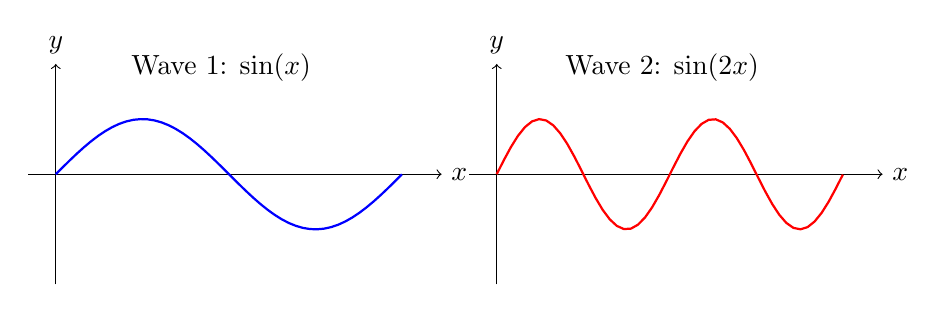
\begin{tikzpicture}[scale=0.7]
        % Wave 1
        \begin{scope}[xshift=0cm]
            \draw[->] (-0.5,0) -- (7,0) node[right] {$x$};
            \draw[->] (0,-2) -- (0,2) node[above] {$y$};
            \draw[thick, blue] plot[domain=0:6.28, samples=50] (\x, {sin(\x r)});
            \node[above] at (3,1.5) {Wave 1: $\sin(x)$};
        \end{scope}

        % Wave 2
        \begin{scope}[xshift=8cm]
            \draw[->] (-0.5,0) -- (7,0) node[right] {$x$};
            \draw[->] (0,-2) -- (0,2) node[above] {$y$};
            \draw[thick, red] plot[domain=0:6.28, samples=50] (\x, {sin(2*\x r)});
            \node[above] at (3,1.5) {Wave 2: $\sin(2x)$};
        \end{scope}
    \end{tikzpicture}
\end{center}

We combine these two waves by weighting the first wave by 1.5 and the second wave by 0.5. $\text{Combined Wave} = 1.5 \cdot \sin(x) + 0.5 \cdot \sin(2x)$. Draw the combined waves.

\begin{center}
\begin{tikzpicture}[scale=0.7]
    % Draw axes
    \draw[->] (-0.5,0) -- (7,0) node[right] {$x$};
    \draw[->] (0,-2) -- (0,2) node[above] {$y$};

    % Draw the composite wave
    %\draw[thick] plot[domain=0:6.28, samples=100]
    %    (\x, {1.5*sin(\x r) + 0.5*sin(2*\x r)});

    % Label
    \node[above] at (3,2) {Combined Wave};
\end{tikzpicture}
\end{center}

\item The Fourier transform is a reverse operation: it decomposes, not combines, waves into basic waves. The waves are continuous functions. But we can discretize them for computation as follows:

\begin{center}
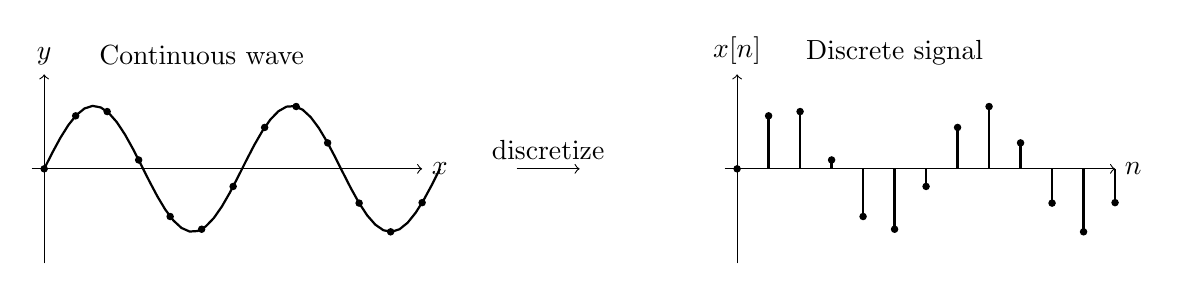
\begin{tikzpicture}[scale=0.8]
    % Original continuous wave
    \begin{scope}[xshift=-1cm]
        \draw[->] (-0.2,0) -- (6,0) node[right] {$x$};
        \draw[->] (0,-1.5) -- (0,1.5) node[above] {$y$};
        \draw[thick] plot[domain=0:2*pi, samples=50] (\x, {sin(2*\x r)});
        \node[above] at (2.5,1.5) {Continuous wave};

        % Draw sample points
        \foreach \x in {0,0.5,...,6} {
            \filldraw[black] (\x,{sin(2*\x r)}) circle (0.05);
        }
    \end{scope}

    % Arrow indicating discretization
    \draw[->] (6.5,0) -- (7.5,0);
    \node[above] at (7,0) {discretize};

    % Discretized signal
    \begin{scope}[xshift=10cm]
        \draw[->] (-0.2,0) -- (6,0) node[right] {$n$};
        \draw[->] (0,-1.5) -- (0,1.5) node[above] {$x[n]$};

        % Draw stems
        \foreach \x [count=\i from 0] in {0,0.5,...,6} {
            \draw[thick] (\i*0.5,0) -- (\i*0.5,{sin(2*\x r)});
            \filldraw[black] (\i*0.5,{sin(2*\x r)}) circle (0.05);
        }
        \node[above] at (2.5,1.5) {Discrete signal};
    \end{scope}
\end{tikzpicture}
\end{center}

This results in a vector of values $[10, 80, 10, 80, 10, 80, 10, 80]$. Now, let's create a discretized mixed wave $Z$ from $X$ and $Y$ as follows

\begin{align}
Z = X + Y = [10, 90, 30, 90, 10, 70, -10, 70, 10]
\end{align}
where
\begin{align}
X = [10, 80, 10, 80, 10, 80, 10, 80, 10], \quad
Y = [0, 10, 20, 10, 0, -10, -20, -10, 0]
\end{align}

(a) If we apply a kernel $K = [-1, 1, -1]$ to this signal, what will be the resulting signal? What kind of frequencies will this kernel emphasize?
\vspace{4em}

(c) If we apply a kernel $K = [1, 1, 1]$ to this signal, what will be the resulting signal? What kind of frequencies will this kernel emphasize?
\vspace{2em}

\clearpage

\item Just as 1D signals can be decomposed into sine waves, 2D images can be decomposed into 2D waves as follows. The Fourier transform can be applied to 2D images to decompose them into a sum of 2D waves.

\begin{center}
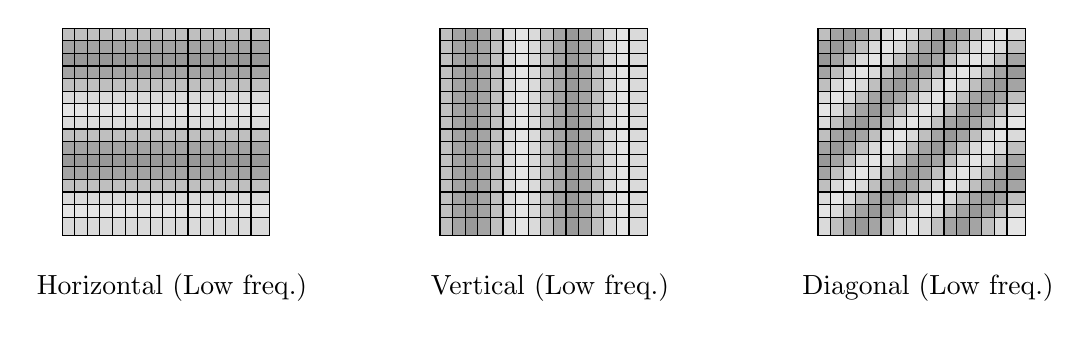
\begin{tikzpicture}[scale=0.8]
    % Horizontal wave (low frequency)
    \begin{scope}[xshift=0cm]
        \foreach \i in {0,...,15} {
            \foreach \j in {0,...,15} {
                \pgfmathsetmacro{\value}{50 + 30*sin(\j*45)}
                \node[rectangle, draw, minimum size=0.2cm, fill=gray!\value] at (\i*0.2, -\j*0.2) {};
            }
        }
        \node[below] at (1.6,-3.6) {Horizontal (Low freq.)};
    \end{scope}

    % Vertical wave
    \begin{scope}[xshift=6cm]
        \foreach \i in {0,...,15} {
            \foreach \j in {0,...,15} {
                \pgfmathsetmacro{\value}{50 + 30*sin(\i*45)}
                \node[rectangle, draw, minimum size=0.2cm, fill=gray!\value] at (\i*0.2, -\j*0.2) {};
            }
        }
        \node[below] at (1.6,-3.6) {Vertical (Low freq.)};
    \end{scope}

    % Diagonal wave
    \begin{scope}[xshift=12cm]
        \foreach \i in {0,...,15} {
            \foreach \j in {0,...,15} {
                \pgfmathsetmacro{\value}{50 + 30*sin((\i+\j)*45)}
                \node[rectangle, draw, minimum size=0.2cm, fill=gray!\value] at (\i*0.2, -\j*0.2) {};
            }
        }
        \node[below] at (1.6,-3.6) {Diagonal (Low freq.)};
    \end{scope}
\end{tikzpicture}

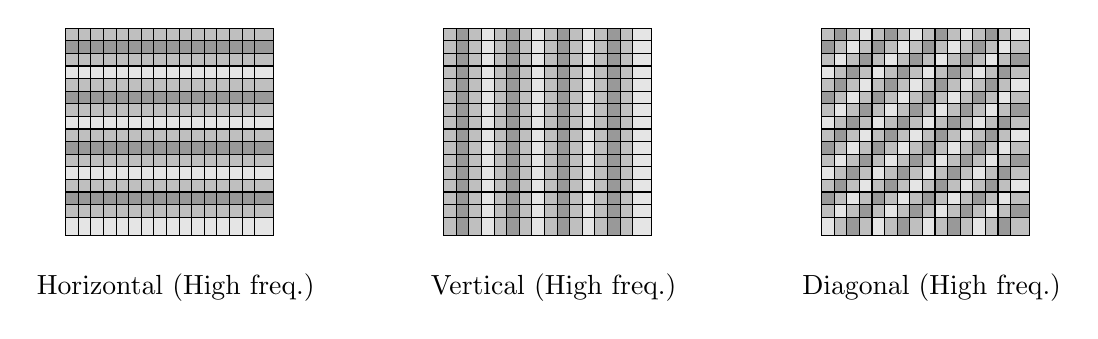
\begin{tikzpicture}[scale=0.8]
    % Horizontal wave (high frequency)
    \begin{scope}[xshift=0cm]
        \foreach \i in {0,...,15} {
            \foreach \j in {0,...,15} {
                \pgfmathsetmacro{\value}{50 + 30*sin(\j*90)}
                \node[rectangle, draw, minimum size=0.2cm, fill=gray!\value] at (\i*0.2, -\j*0.2) {};
            }
        }
        \node[below] at (1.6,-3.6) {Horizontal (High freq.)};
    \end{scope}

    % Vertical wave (high frequency)
    \begin{scope}[xshift=6cm]
        \foreach \i in {0,...,15} {
            \foreach \j in {0,...,15} {
                \pgfmathsetmacro{\value}{50 + 30*sin(\i*90)}
                \node[rectangle, draw, minimum size=0.2cm, fill=gray!\value] at (\i*0.2, -\j*0.2) {};
            }
        }
        \node[below] at (1.6,-3.6) {Vertical (High freq.)};
    \end{scope}

    % Diagonal wave (high frequency)
    \begin{scope}[xshift=12cm]
        \foreach \i in {0,...,15} {
            \foreach \j in {0,...,15} {
                \pgfmathsetmacro{\value}{50 + 30*sin((\i+\j)*90)}
                \node[rectangle, draw, minimum size=0.2cm, fill=gray!\value] at (\i*0.2, -\j*0.2) {};
            }
        }
        \node[below] at (1.6,-3.6) {Diagonal (High freq.)};
    \end{scope}
\end{tikzpicture}
\end{center}

Now, consider this checkerboard pattern on the left. Mark where you expect the highest magnitudes in the Fourier transform grid. The dashed circles represent the basis 2D waves in the Fourier domain.

\begin{center}
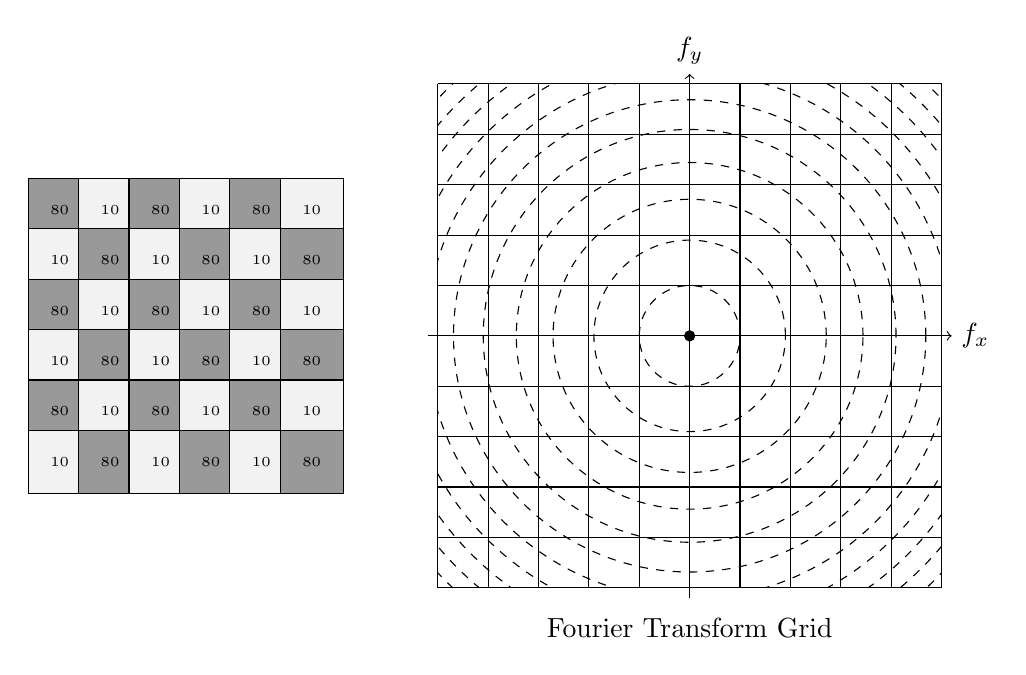
\begin{tikzpicture}[scale=0.8]
    % Create 6x6 checkerboard
    \begin{scope}[xshift=0cm, yshift=2cm]
    \foreach \i in {0,...,5} {
        \foreach \j in {0,...,5} {
            \pgfmathsetmacro{\value}{ifthenelse(mod(\i+\j,2)==0, 80, 10)}
            \node[rectangle, draw, minimum size=0.8cm, fill=gray!\value] at (\i*0.8, -\j*0.8) {\tiny \value};
        }
        }
    \end{scope}
    \begin{scope}[xshift=10cm,scale=0.8]
        % Draw main grid 7x7
        \draw (-5,-5) grid (5,5);

        % Draw coordinate axes
        \draw[->] (-5.2,0) -- (5.2,0) node[right] {$f_x$};
        \draw[->] (0,-5.2) -- (0,5.2) node[above] {$f_y$};

        % Add center dot
        \filldraw (0,0) circle (0.1);
        \node at (0,-5.8) {Fourier Transform Grid};

        % Add circles with radius up to 4.2 (to reach corners)
        % But clip them to show only within the grid
        \begin{scope}
            \clip (-5,-5) rectangle (5,5);
            \foreach \k in {1, ..., 40} {
                \pgfmathsetmacro{\r}{1 * (1 - 0.9^\k) / (1 - 0.9)}
                \draw[dashed] (0,0) circle (\r);
            }
        \end{scope}
    \end{scope}
\end{tikzpicture}
\end{center}

\item The image can be mapped to the Fourier transform grid (called frequency domain). We can also map it back to the original image domain (called spatial domain). Thus, we can manipulate the image in the frequency domain to remove some waves from the original image.
If we want to keep only the low-frequency components of the checkerboard pattern, what regions of the Fourier transform grid should we set to zero?

\end{enumerate}

\clearpage

\section*{Weisfeiler-Lehman Test}

A neural network's job is often graph classification (e.g., is this molecule toxic?). To do this, the network must be able to distinguish between two different graphs.

Below are two molecules (Graph $G_1$ and Graph $G_2$). They consist of atoms labeled \textbf{A} and \textbf{B}. If we present this to a neural network that simply counts labels, it will likely not be able to distinguish between the two graphs.

% --- PART 1 ---
\begin{center}
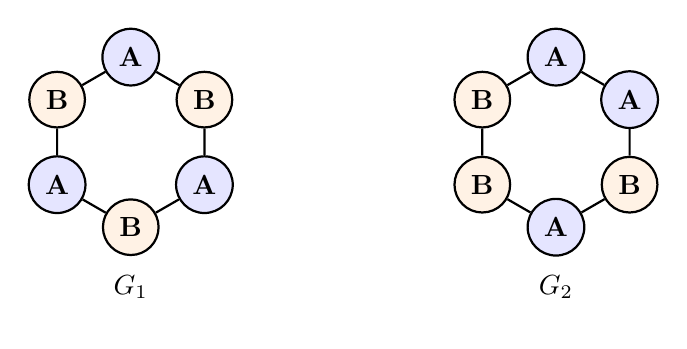
\begin{tikzpicture}[scale=0.9, every node/.style={circle, draw=black, thick, minimum size=0.7cm, font=\bfseries}]

    % Graph 1: Perfect Alternating Hexagon
    \def\R{1.2}
    \node[fill=blue!10]   (1) at (90:\R)  {A};
    \node[fill=orange!10] (2) at (30:\R)  {B};
    \node[fill=blue!10]   (3) at (-30:\R) {A};
    \node[fill=orange!10] (4) at (-90:\R) {B};
    \node[fill=blue!10]   (5) at (-150:\R){A};
    \node[fill=orange!10] (6) at (150:\R) {B};
    \draw[thick] (1) -- (2) -- (3) -- (4) -- (5) -- (6) -- (1);
    \node[draw=none, below=1.4cm] at (0,0) {\textbf{$G_1$}};

    % Graph 2: Clumped Labels
    \begin{scope}[xshift=6cm]
        \node[fill=blue!10]   (1) at (90:\R)  {A};
        \node[fill=blue!10]   (2) at (30:\R)  {A};
        \node[fill=orange!10] (3) at (-30:\R) {B};
        \node[fill=blue!10]   (4) at (-90:\R) {A};
        \node[fill=orange!10] (5) at (-150:\R){B};
        \node[fill=orange!10] (6) at (150:\R) {B};
        \draw[thick] (1) -- (2) -- (3) -- (4) -- (5) -- (6) -- (1);
        \node[draw=none, below=1.4cm] at (0,0) {\textbf{$G_2$}};
    \end{scope}
\end{tikzpicture}
\end{center}

\subsection*{Part 1: Distinguishing Labeled Graphs}

Let's work up a solution step by step. Since counting labels (global pooling) doesn't work, let's look at the \textbf{local structure} around each node.

\vspace{0.3cm}

\textbf{Step 1: Message Passing.}
Create a \textbf{signature} for every node: `(My Label, \{Neighbor Labels\})`.

\begin{minipage}{0.48\textwidth}
\textbf{Graph $G_1$ Signatures:}
\begin{itemize}[leftmargin=*]
    \item Any Node A: \texttt{(A, \{B, B\})}
    \item Any Node B: \texttt{(B, \{A, A\})}
\end{itemize}
\end{minipage}
\hfill
\begin{minipage}{0.48\textwidth}
\textbf{Graph $G_2$ Signatures:}
\begin{itemize}[leftmargin=*]
    \item Top Node (A): \underline{\hspace{4cm}}
    \item Top-Right Node (A): \underline{\hspace{3.2cm}}
    \item Bottom Node (A): \texttt{(A, \{B, B\})}
\end{itemize}
\end{minipage}

\vspace{0.3cm}

\textbf{Step 2: Compression (Hashing).}
Assign a unique ID to every unique signature found across both graphs.

\begin{center}
\begin{tabular}{l c l | l c l}
    \toprule
    Signature & $\rightarrow$ & ID & Signature & $\rightarrow$ & ID \\
    \midrule
    (A, \{B, B\}) & $\rightarrow$ & \textbf{1} & (B, \{A, B\}) & $\rightarrow$ & \textbf{4} \\
    (B, \{A, A\}) & $\rightarrow$ & \textbf{2} & (A, \{A, A\}) & $\rightarrow$ & \textbf{5} \\
    (A, \{A, B\}) & $\rightarrow$ & \textbf{3} & (B, \{B, B\}) & $\rightarrow$ & \textbf{6} \\
    \bottomrule
\end{tabular}
\end{center}

\textbf{Step 3: Rewrite with Colors.}
List the set of Color IDs present in each graph.
\begin{itemize}
    \item \textbf{$G_1$ Colors:} \{ 1, 1, 1, 2, 2, 2 \}
    \item \textbf{$G_2$ Colors:} \{ \underline{\hspace{0.5cm}}, \underline{\hspace{0.5cm}}, \underline{\hspace{0.5cm}}, \underline{\hspace{0.5cm}}, \underline{\hspace{0.5cm}}, \underline{\hspace{0.5cm}} \}
\end{itemize}
\textbf{Conclusion:} Are the sets of colors different? \textbf{[ Yes / No ]}

\clearpage
\subsubsection*{Exercise B: Structural Difference}
Below are graphs $G_3$ (Line) and $G_4$ (Star). Both have \textbf{5 Nodes} (2 As, 3 Bs).

\begin{center}
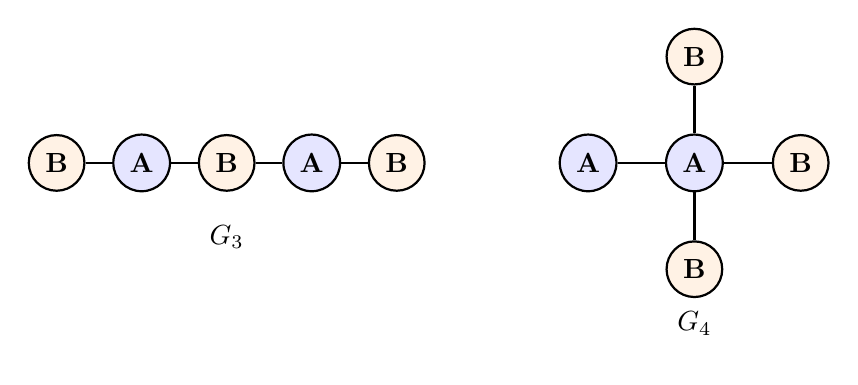
\begin{tikzpicture}[scale=0.9, every node/.style={circle, draw=black, thick, minimum size=0.7cm, font=\bfseries}]
    % Graph 3: Linear Chain
    \node[fill=orange!10] (1) at (0,0) {B};
    \node[fill=blue!10]   (2) at (1.2,0) {A};
    \node[fill=orange!10] (3) at (2.4,0) {B};
    \node[fill=blue!10]   (4) at (3.6,0) {A};
    \node[fill=orange!10] (5) at (4.8,0) {B};
    \draw[thick] (1)--(2)--(3)--(4)--(5);
    \node[draw=none, below=0.5cm] at (2.4,0) {\textbf{$G_3$}};

    % Graph 4: Star
    \begin{scope}[xshift=9cm, yshift=0cm]
        \node[fill=blue!10] (C) at (0,0) {A};
        \node[fill=orange!10] (N) at (0,1.5) {B};
        \node[fill=orange!10] (S) at (0,-1.5) {B};
        \node[fill=orange!10] (E) at (1.5,0) {B};
        \node[fill=blue!10]   (W) at (-1.5,0) {A};
        \draw[thick] (N)--(C)--(S); \draw[thick] (W)--(C)--(E);
        \node[draw=none, below=1.6cm] at (0,0) {\textbf{$G_4$}};
    \end{scope}
\end{tikzpicture}
\end{center}

\textbf{Task:} Fill in the signatures `(My Label, \{Neighbors\})` for all nodes.

\begin{minipage}{0.48\textwidth}
\textbf{Graph $G_3$ (Line):}
\begin{itemize}[leftmargin=*]
    \item Left B: \underline{\hspace{3.5cm}}
    \item Left A: \underline{\hspace{3.5cm}}
    \item Middle B: \underline{\hspace{3.5cm}}
    \item Right A: \underline{\hspace{3.5cm}}
    \item Right B: \underline{\hspace{3.5cm}}
\end{itemize}
\end{minipage}
\hfill
\begin{minipage}{0.48\textwidth}
\textbf{Graph $G_4$ (Star):}
\begin{itemize}[leftmargin=*]
    \item Center A: \underline{\hspace{3.5cm}}
    \item Left A: \underline{\hspace{3.5cm}}
    \item Top B: \underline{\hspace{3.5cm}}
    \item Right B: \underline{\hspace{3.5cm}}
    \item Bottom B: \underline{\hspace{3.5cm}}
\end{itemize}
\end{minipage}

\textbf{Compare:} Does $G_4$ generate a signature that is completely impossible in $G_3$? \textbf{[ Yes / No ]}

% --- PART 2 ---
\subsection*{Part 2: Identifying Isomorphic Graphs (Unlabeled)}

Sometimes different drawings represent the same graph. A GNN should map these to the same embedding.
Consider $H_1$ (The House) and $H_2$ (Pentagon w/ Chord).

\begin{center}
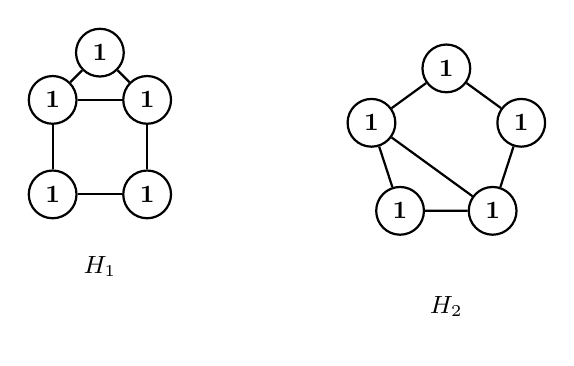
\begin{tikzpicture}[scale=1.0, every node/.style={circle, draw=black, thick, minimum size=0.6cm, font=\small\bfseries}]

    % Graph H1: The House
    \node (1) at (0,0) {1};
    \node (2) at (1.2,0) {1};
    \node (3) at (1.2,1.2) {1};
    \node (4) at (0,1.2) {1};
    \node (5) at (0.6, 1.8) {1};
    \draw[thick] (1)--(2)--(3)--(4)--(1);
    \draw[thick] (4)--(5)--(3);
    \node[draw=none, below=0.5cm] at (0.6, 0) {\textbf{$H_1$}};

    % Graph H2: Pentagon with Chord
    \begin{scope}[xshift=5cm, yshift=0.6cm]
        \def\R{1.0}
        \node (A) at (90:\R) {1};
        \node (B) at (18:\R) {1};
        \node (C) at (-54:\R) {1};
        \node (D) at (234:\R) {1};
        \node (E) at (162:\R) {1};
        \draw[thick] (A)--(B)--(C)--(D)--(E)--(A);
        \draw[thick] (E)--(C);
        \node[draw=none, below=1.1cm] at (0, -0.5) {\textbf{$H_2$}};
    \end{scope}
\end{tikzpicture}
\end{center}

Since there are no node labels (A or B), we initialize \textbf{all nodes} with the label "\textbf{1}". Perform the same Message Passing process as Part 1.
Create signatures for every node: \texttt{(My Label, \{Neighbor Labels\})}.

\begin{center}
\renewcommand{\arraystretch}{1.5}
\begin{tabular}{|c|c|c|}
    \hline
    \textbf{Signature Found} & \textbf{Number of nodes in $H_1$} & \textbf{Number of nodes in $H_2$} \\
    \hline
    \texttt{(1, \{1, 1\})} & \hspace{3cm} & \hspace{3cm} \\
    \hline
    \texttt{(1, \{1, 1, 1\})} & \hspace{3cm} & \hspace{3cm} \\
    \hline
\end{tabular}
\end{center}

\textbf{Conclusion:} Compare the counts in the table.
\begin{enumerate}
    \item Are the "histograms" (counts of signatures) identical? \textbf{[ Yes / No ]}
    \item If they are identical, the WL test cannot distinguish them (Likely Isomorphic).
\end{enumerate}

\vspace{0.5cm}

% --- PART 3 ---
\subsection*{Part 3: When WL Fails}
Consider $L_1$ (Hexagon) and $L_2$ (Two Triangles). All labels "1".

\begin{center}
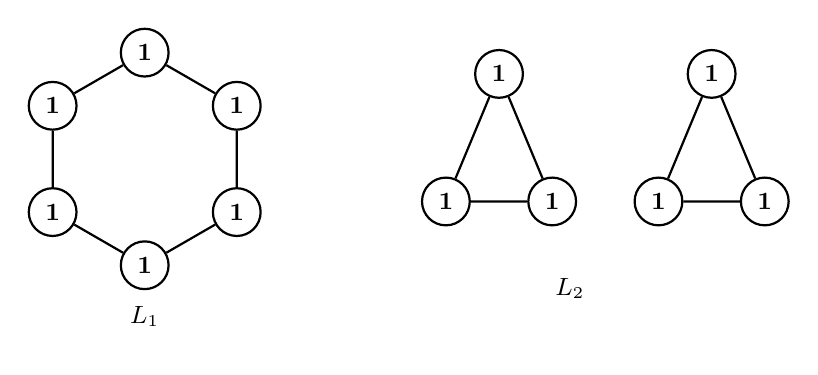
\begin{tikzpicture}[scale=0.9, every node/.style={circle, draw=black, thick, minimum size=0.6cm, font=\small\bfseries}]
    % Graph L1: Hexagon
    \def\R{1.5}
    \node (1) at (90:\R) {1};
    \node (2) at (30:\R) {1};
    \node (3) at (-30:\R) {1};
    \node (4) at (-90:\R) {1};
    \node (5) at (-150:\R) {1};
    \node (6) at (150:\R) {1};
    \draw[thick] (1)--(2)--(3)--(4)--(5)--(6)--(1);
    \node[draw=none, below=1.6cm] at (0,0) {\textbf{$L_1$}};

    % Graph L2: Two Triangles
    \begin{scope}[xshift=5cm]
        \node (A1) at (0,1.2) {1};
        \node (B1) at (-0.75,-0.6) {1};
        \node (C1) at (0.75,-0.6) {1};
        \draw[thick] (A1)--(B1)--(C1)--(A1);
        \begin{scope}[xshift=3.0cm]
             \node (A2) at (0,1.2) {1};
             \node (B2) at (-0.75,-0.6) {1};
             \node (C2) at (0.75,-0.6) {1};
             \draw[thick] (A2)--(B2)--(C2)--(A2);
        \end{scope}
        \node[draw=none, below=0.8cm] at (1.0, -0.5) {\textbf{$L_2$}};
    \end{scope}
\end{tikzpicture}
\end{center}

Perform the same Message Passing process as Part 1, and fill in the table below.

\begin{center}
\begin{tabular}{|c|c|c|}
    \hline
    \textbf{Signature Found} & \textbf{Number of nodes in $L_1$} & \textbf{Number of nodes in $L_2$} \\
    \hline
    \texttt{(1, \{1, 1\})} & \hspace{3cm} & \hspace{3cm} \\
    \hline
\end{tabular}
\end{center}

See if the counts in the table are identical (i.e., the WL test cannot distinguish them) or not (i.e., the WL test can distinguish them). What does this tell us about the power of the WL test?

\clearpage

% --- PART 4 ---
\section*{Part 4: The Neural Connection (Mapping WL to GCN)}

We've worked through the Weisfeiler-Lehman (WL) test by hand! Now let's see how this classic, step-by-step coloring idea shows up inside a Graph Convolutional Network (GCN). You can think of a GCN as a kind of ``smooth'' or ``continuous'' version of the WL process.

A typical GCN layer updates the features $h_v$ of node $v$ with the following recipe:

\[
h_v^{(new)} = \sigma \left( W \cdot \sum_{u \in \mathcal{N}(v) \cup \{v\}} \frac{1}{\sqrt{d_v d_u}} h_u \right)
\]

\textbf{Notation:}
\begin{itemize}
    \item $h_v$ = feature vector of node $v$ (e.g., a vector like $[0.2, 1.5, -0.3]$)
    \item $\mathcal{N}(v)$ = the set of neighbors of node $v$
    \item $d_v$ = degree of node $v$ (number of neighbors)
    \item $W$ = weight matrix (learnable parameters that transform features)
    \item $\sigma$ = activation function (e.g., ReLU, sigmoid; adds nonlinearity)
\end{itemize}

\vspace{0.3cm}

Let's make some connections between the parts of this GCN equation and the steps you took in the WL test:

\begin{enumerate}
    \item \textbf{The ``Collection'' Step:} In the WL test, you ``collected'' the labels of neighbors into a bag (a multiset), like \{A, B, B\}. Which part of the formula above does something similar? \\
    \vspace{0.5cm}
    \textbf{Answer:} \underline{\hspace{8cm}}

    \item \textbf{The ``Hashing'' Step:} Remember how the WL test assigned a new color (ID) by looking up the unique neighbor patterns? In neural nets, we don't use lookup tables---instead, which component here ``mixes and matches'' those patterns into new features? \\
    \vspace{0.5cm}
    \textbf{Answer:} \underline{\hspace{8cm}}

    \item \textbf{The ``Color'' Step:} While the WL test spit out new integer colors (like 3, 7, or 11), GCNs make continuous vectors. The final step is deciding when a neuron ``lights up'' for a certain pattern---which we do with a nonlinear activation! \\
    \vspace{0.5cm}
    \textbf{Answer:} \underline{\hspace{8cm}}
\end{enumerate}

\end{document}